\section{Frame Assembly}
The full frame and chassis of the vehicle were provided, however some modifications were necessary in order to incorporate the new design which allowed the 30:1 reduction box output shaft be coupled to the drive shaft of the drive box using a flexible coupling. In addition to the horizontal cross member, four vertical members were placed on the corners of the horizontal crossers to direct forces up through the rest of the frame, thus reducing the reliance on the welds to hold the weight of the vehicle. Furthermore, aluminum inserts were welded to the frame hole cutouts, in which brass bushings were pressed. The aluminum insert had a tapped hole with a grease nipple and a shoulder to separate both brass bushings, allowing grease to be put between the pivot and bushings. The frame assembly can be seen in Figure~\ref{fig:battery_rack_and_frame_mount_drw}, and highlights both the horizontal and vertical supports.   
\begin{figure}[h]
\centering
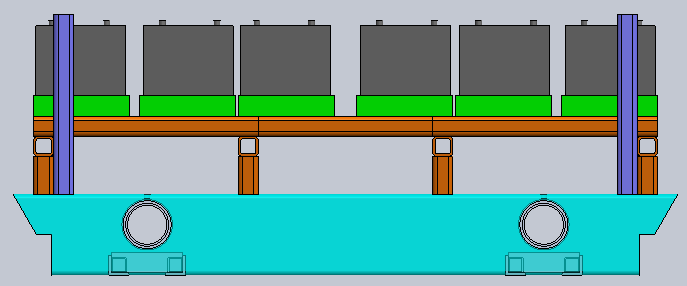
\includegraphics[width=0.8\linewidth]{./images/battery_rack_and_frame_mount_drw}
\caption{Frame Assembly Including Battery Rack and Frame Extension}
\label{fig:battery_rack_and_frame_mount_drw}
\end{figure}
\subsection{Design Constraints and Functional Requirements}
The design of the frame insert was constrained by the length of the vehicle, and needed to be made out rectangular tubing with a large enough height to accomodate the output hole for the pivot. Since the frame shell could not be removed, the frame insert needed to be custom made to fit into the space where the old horizontal members were cut out. Many attempts were made at modelling the modifications, however the greatest success came from creating a cardboard template to mark up the tubing after which the desired geometry was finally cut out. The vertical supports needed to be placed on top of the rectangular tubing and extend into the top portion of the frame where it was welded. Furthermore, The entire addition needed to be made out of the same grade of aluminum as the frame was to be weldable.  

\subsection{Analysis and Design}
The output hole in the frame needed to be raised by 10\,cm, however the existing frame member was 2x2x1/8'' rectangular tubing. In order to raise the height of the output hole it was required that 2x8x3/16'' rectangular tubing was used. Under the assumed loading conditions, hand calculations showed that this cross sectional area could withstand the bending moment and shear induced by the vertical force at the center of the circular bushing insert. Additionally, the material required was 6061 aluminum to match the material used for the rest of the frame. 
\begin{figure}[H]
\centering
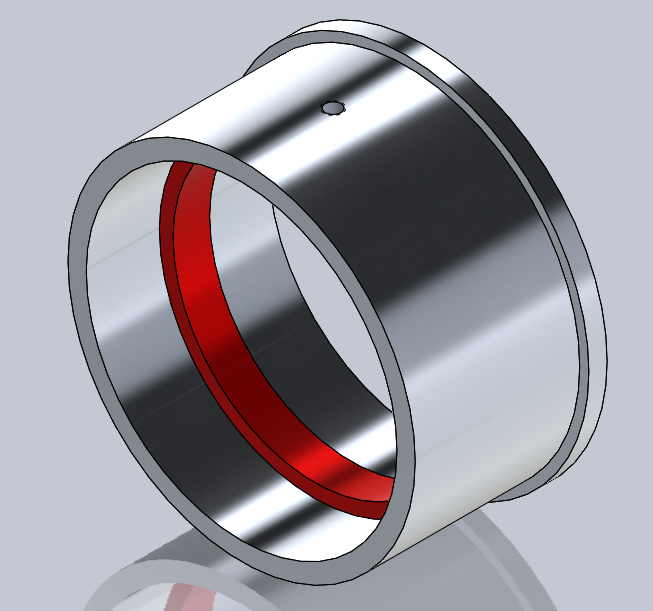
\includegraphics[width=0.25\linewidth]{./images/frame_insert_iso_rndr}
\caption{Aluminum Frame Insert With Flange}
\label{fig:frame_insert_iso_rndr}
\end{figure}

A cylindrical, aluminum frame insert needed to be welded inside the hole in the frame extension. The insert needed to have a large enough inside diameter to have an interference fit with the brass bushings. The insert had a cylindrical shoulder 1/4'' thick with a diameter 1/8'' less than the inside diameter of the insert. The flanged section was located in the middle of the insert and allowed for the separation of the two bushing sections to be able to apply grease from the grease nipple located on the outside of the insert. An illustration of the aluminum frame insert can be seen in Figure~\ref{fig:frame_insert_iso_rndr}.

Under the assumption that the pivot would be rotating at a continuous speed of 15\,mm/s, the wear life of the bearing was estimated to be $18500\times w\,\text{hours}$ where $w$ was the desired wear thickness of the bushing. It was assumed that the interior of the bushing would wear quicker than the face of the bushing in contact with the pivot and the travel limiter. Therefore the thickness of the bushing extending past the frame was chosen to be 1/8'', and the wear of the bushing before replacement was also selected to be 1/8''. The brass tubing was chosen because it required minimal machining to achieve the required dimensions. 